% Options for packages loaded elsewhere
\PassOptionsToPackage{unicode}{hyperref}
\PassOptionsToPackage{hyphens}{url}
%
\documentclass[
]{article}
\title{Homework 1}
\author{}
\date{\vspace{-2.5em}Winter 2022}

\usepackage{amsmath,amssymb}
\usepackage{lmodern}
\usepackage{iftex}
\ifPDFTeX
  \usepackage[T1]{fontenc}
  \usepackage[utf8]{inputenc}
  \usepackage{textcomp} % provide euro and other symbols
\else % if luatex or xetex
  \usepackage{unicode-math}
  \defaultfontfeatures{Scale=MatchLowercase}
  \defaultfontfeatures[\rmfamily]{Ligatures=TeX,Scale=1}
\fi
% Use upquote if available, for straight quotes in verbatim environments
\IfFileExists{upquote.sty}{\usepackage{upquote}}{}
\IfFileExists{microtype.sty}{% use microtype if available
  \usepackage[]{microtype}
  \UseMicrotypeSet[protrusion]{basicmath} % disable protrusion for tt fonts
}{}
\makeatletter
\@ifundefined{KOMAClassName}{% if non-KOMA class
  \IfFileExists{parskip.sty}{%
    \usepackage{parskip}
  }{% else
    \setlength{\parindent}{0pt}
    \setlength{\parskip}{6pt plus 2pt minus 1pt}}
}{% if KOMA class
  \KOMAoptions{parskip=half}}
\makeatother
\usepackage{xcolor}
\IfFileExists{xurl.sty}{\usepackage{xurl}}{} % add URL line breaks if available
\IfFileExists{bookmark.sty}{\usepackage{bookmark}}{\usepackage{hyperref}}
\hypersetup{
  pdftitle={Homework 1},
  hidelinks,
  pdfcreator={LaTeX via pandoc}}
\urlstyle{same} % disable monospaced font for URLs
\usepackage[margin=1in]{geometry}
\usepackage{color}
\usepackage{fancyvrb}
\newcommand{\VerbBar}{|}
\newcommand{\VERB}{\Verb[commandchars=\\\{\}]}
\DefineVerbatimEnvironment{Highlighting}{Verbatim}{commandchars=\\\{\}}
% Add ',fontsize=\small' for more characters per line
\usepackage{framed}
\definecolor{shadecolor}{RGB}{248,248,248}
\newenvironment{Shaded}{\begin{snugshade}}{\end{snugshade}}
\newcommand{\AlertTok}[1]{\textcolor[rgb]{0.94,0.16,0.16}{#1}}
\newcommand{\AnnotationTok}[1]{\textcolor[rgb]{0.56,0.35,0.01}{\textbf{\textit{#1}}}}
\newcommand{\AttributeTok}[1]{\textcolor[rgb]{0.77,0.63,0.00}{#1}}
\newcommand{\BaseNTok}[1]{\textcolor[rgb]{0.00,0.00,0.81}{#1}}
\newcommand{\BuiltInTok}[1]{#1}
\newcommand{\CharTok}[1]{\textcolor[rgb]{0.31,0.60,0.02}{#1}}
\newcommand{\CommentTok}[1]{\textcolor[rgb]{0.56,0.35,0.01}{\textit{#1}}}
\newcommand{\CommentVarTok}[1]{\textcolor[rgb]{0.56,0.35,0.01}{\textbf{\textit{#1}}}}
\newcommand{\ConstantTok}[1]{\textcolor[rgb]{0.00,0.00,0.00}{#1}}
\newcommand{\ControlFlowTok}[1]{\textcolor[rgb]{0.13,0.29,0.53}{\textbf{#1}}}
\newcommand{\DataTypeTok}[1]{\textcolor[rgb]{0.13,0.29,0.53}{#1}}
\newcommand{\DecValTok}[1]{\textcolor[rgb]{0.00,0.00,0.81}{#1}}
\newcommand{\DocumentationTok}[1]{\textcolor[rgb]{0.56,0.35,0.01}{\textbf{\textit{#1}}}}
\newcommand{\ErrorTok}[1]{\textcolor[rgb]{0.64,0.00,0.00}{\textbf{#1}}}
\newcommand{\ExtensionTok}[1]{#1}
\newcommand{\FloatTok}[1]{\textcolor[rgb]{0.00,0.00,0.81}{#1}}
\newcommand{\FunctionTok}[1]{\textcolor[rgb]{0.00,0.00,0.00}{#1}}
\newcommand{\ImportTok}[1]{#1}
\newcommand{\InformationTok}[1]{\textcolor[rgb]{0.56,0.35,0.01}{\textbf{\textit{#1}}}}
\newcommand{\KeywordTok}[1]{\textcolor[rgb]{0.13,0.29,0.53}{\textbf{#1}}}
\newcommand{\NormalTok}[1]{#1}
\newcommand{\OperatorTok}[1]{\textcolor[rgb]{0.81,0.36,0.00}{\textbf{#1}}}
\newcommand{\OtherTok}[1]{\textcolor[rgb]{0.56,0.35,0.01}{#1}}
\newcommand{\PreprocessorTok}[1]{\textcolor[rgb]{0.56,0.35,0.01}{\textit{#1}}}
\newcommand{\RegionMarkerTok}[1]{#1}
\newcommand{\SpecialCharTok}[1]{\textcolor[rgb]{0.00,0.00,0.00}{#1}}
\newcommand{\SpecialStringTok}[1]{\textcolor[rgb]{0.31,0.60,0.02}{#1}}
\newcommand{\StringTok}[1]{\textcolor[rgb]{0.31,0.60,0.02}{#1}}
\newcommand{\VariableTok}[1]{\textcolor[rgb]{0.00,0.00,0.00}{#1}}
\newcommand{\VerbatimStringTok}[1]{\textcolor[rgb]{0.31,0.60,0.02}{#1}}
\newcommand{\WarningTok}[1]{\textcolor[rgb]{0.56,0.35,0.01}{\textbf{\textit{#1}}}}
\usepackage{graphicx}
\makeatletter
\def\maxwidth{\ifdim\Gin@nat@width>\linewidth\linewidth\else\Gin@nat@width\fi}
\def\maxheight{\ifdim\Gin@nat@height>\textheight\textheight\else\Gin@nat@height\fi}
\makeatother
% Scale images if necessary, so that they will not overflow the page
% margins by default, and it is still possible to overwrite the defaults
% using explicit options in \includegraphics[width, height, ...]{}
\setkeys{Gin}{width=\maxwidth,height=\maxheight,keepaspectratio}
% Set default figure placement to htbp
\makeatletter
\def\fps@figure{htbp}
\makeatother
\setlength{\emergencystretch}{3em} % prevent overfull lines
\providecommand{\tightlist}{%
  \setlength{\itemsep}{0pt}\setlength{\parskip}{0pt}}
\setcounter{secnumdepth}{-\maxdimen} % remove section numbering
\ifLuaTeX
  \usepackage{selnolig}  % disable illegal ligatures
\fi

\begin{document}
\maketitle

\begin{Shaded}
\begin{Highlighting}[]
\NormalTok{algae }\OtherTok{\textless{}{-}} \FunctionTok{read\_table2}\NormalTok{(}\StringTok{"algaeBloom.txt"}\NormalTok{, }\AttributeTok{col\_names=}
                       \FunctionTok{c}\NormalTok{(}\StringTok{\textquotesingle{}season\textquotesingle{}}\NormalTok{,}\StringTok{\textquotesingle{}size\textquotesingle{}}\NormalTok{,}\StringTok{\textquotesingle{}speed\textquotesingle{}}\NormalTok{,}\StringTok{\textquotesingle{}mxPH\textquotesingle{}}\NormalTok{,}\StringTok{\textquotesingle{}mn02\textquotesingle{}}\NormalTok{,}\StringTok{\textquotesingle{}C1\textquotesingle{}}\NormalTok{,}\StringTok{\textquotesingle{}NO3\textquotesingle{}}\NormalTok{,}\StringTok{\textquotesingle{}NH4\textquotesingle{}}\NormalTok{,}\StringTok{\textquotesingle{}cPO4\textquotesingle{}}\NormalTok{,}\StringTok{\textquotesingle{}PO4\textquotesingle{}}\NormalTok{,}\StringTok{\textquotesingle{}CHla\textquotesingle{}}\NormalTok{,}\StringTok{\textquotesingle{}a1\textquotesingle{}}\NormalTok{,}\StringTok{\textquotesingle{}a2\textquotesingle{}}\NormalTok{,}\StringTok{\textquotesingle{}a3\textquotesingle{}}\NormalTok{,}\StringTok{\textquotesingle{}a4\textquotesingle{}}\NormalTok{,}\StringTok{\textquotesingle{}a5\textquotesingle{}}\NormalTok{,}\StringTok{\textquotesingle{}a6\textquotesingle{}}\NormalTok{,}\StringTok{\textquotesingle{}a7\textquotesingle{}}\NormalTok{), }\AttributeTok{na =} \StringTok{"XXXXXXX"}\NormalTok{)}

\FunctionTok{glimpse}\NormalTok{(algae)}
\end{Highlighting}
\end{Shaded}

\begin{verbatim}
## Rows: 200
## Columns: 18
## $ season <chr> "winter", "spring", "autumn", "spring", "autumn", "winter", "su~
## $ size   <chr> "small", "small", "small", "small", "small", "small", "small", ~
## $ speed  <chr> "medium", "medium", "medium", "medium", "medium", "high", "high~
## $ mxPH   <dbl> 8.00, 8.35, 8.10, 8.07, 8.06, 8.25, 8.15, 8.05, 8.70, 7.93, 7.7~
## $ mn02   <dbl> 9.8, 8.0, 11.4, 4.8, 9.0, 13.1, 10.3, 10.6, 3.4, 9.9, 10.2, 11.~
## $ C1     <dbl> 60.80, 57.75, 40.02, 77.36, 55.35, 65.75, 73.25, 59.07, 21.95, ~
## $ NO3    <dbl> 6.238, 1.288, 5.330, 2.302, 10.416, 9.248, 1.535, 4.990, 0.886,~
## $ NH4    <dbl> 578.00, 370.00, 346.67, 98.18, 233.70, 430.00, 110.00, 205.67, ~
## $ cPO4   <dbl> 105.00, 428.75, 125.67, 61.18, 58.22, 18.25, 61.25, 44.67, 36.3~
## $ PO4    <dbl> 170.00, 558.75, 187.06, 138.70, 97.58, 56.67, 111.75, 77.43, 71~
## $ CHla   <dbl> 50.000, 1.300, 15.600, 1.400, 10.500, 28.400, 3.200, 6.900, 5.5~
## $ a1     <dbl> 0.0, 1.4, 3.3, 3.1, 9.2, 15.1, 2.4, 18.2, 25.4, 17.0, 16.6, 32.~
## $ a2     <dbl> 0.0, 7.6, 53.6, 41.0, 2.9, 14.6, 1.2, 1.6, 5.4, 0.0, 0.0, 0.0, ~
## $ a3     <dbl> 0.0, 4.8, 1.9, 18.9, 7.5, 1.4, 3.2, 0.0, 2.5, 0.0, 0.0, 0.0, 2.~
## $ a4     <dbl> 0.0, 1.9, 0.0, 0.0, 0.0, 0.0, 3.9, 0.0, 0.0, 2.9, 0.0, 0.0, 0.0~
## $ a5     <dbl> 34.2, 6.7, 0.0, 1.4, 7.5, 22.5, 5.8, 5.5, 0.0, 0.0, 1.2, 0.0, 1~
## $ a6     <dbl> 8.3, 0.0, 0.0, 0.0, 4.1, 12.6, 6.8, 8.7, 0.0, 0.0, 0.0, 0.0, 0.~
## $ a7     <dbl> 0.0, 2.1, 9.7, 1.4, 1.0, 2.9, 0.0, 0.0, 0.0, 1.7, 6.0, 1.5, 2.1~
\end{verbatim}

\begin{Shaded}
\begin{Highlighting}[]
\FunctionTok{dim}\NormalTok{(algae)}
\end{Highlighting}
\end{Shaded}

\begin{verbatim}
## [1] 200  18
\end{verbatim}

\begin{enumerate}
\def\labelenumi{\arabic{enumi}.}
\tightlist
\item
  Descriptive summary statistics (10 pts in total) Given the lack of
  further information on the problem domain, it is wise to investigate
  some of the statistical properties of the data, so as to get a better
  grasp of the problem. It is always a good idea to start our analysis
  with some kind of exploratory data analysis. A first idea of the
  statistical properties of the data can be obtained through a summary
  of its descriptive statistics.
\end{enumerate}

\begin{enumerate}
\def\labelenumi{\alph{enumi}.}
\tightlist
\item
  Count the number of observations in each size using summarise() in
  dplyr.
\end{enumerate}

\begin{Shaded}
\begin{Highlighting}[]
\NormalTok{algae }\SpecialCharTok{\%\textgreater{}\%}
  \FunctionTok{group\_by}\NormalTok{(size) }\SpecialCharTok{\%\textgreater{}\%}
    \FunctionTok{summarise}\NormalTok{(}\AttributeTok{n =} \FunctionTok{n}\NormalTok{())}
\end{Highlighting}
\end{Shaded}

\begin{verbatim}
## # A tibble: 3 x 2
##   size       n
##   <chr>  <int>
## 1 large     45
## 2 medium    84
## 3 small     71
\end{verbatim}

\begin{enumerate}
\def\labelenumi{\alph{enumi}.}
\setcounter{enumi}{1}
\tightlist
\item
  Are there missing values? (2 pts) Calculate the mean and variance of
  each chemical (Ignore a1 through a7). (1 pts) What do you notice about
  the magnitude of the two quantities for different chemicals?
\end{enumerate}

\begin{Shaded}
\begin{Highlighting}[]
\FunctionTok{summary}\NormalTok{(algae)}
\end{Highlighting}
\end{Shaded}

\begin{verbatim}
##     season              size              speed                mxPH     
##  Length:200         Length:200         Length:200         Min.   :5.60  
##  Class :character   Class :character   Class :character   1st Qu.:7.70  
##  Mode  :character   Mode  :character   Mode  :character   Median :8.06  
##                                                           Mean   :8.01  
##                                                           3rd Qu.:8.40  
##                                                           Max.   :9.70  
##                                                           NA's   :1     
##       mn02             C1             NO3             NH4       
##  Min.   : 1.50   Min.   :  0.2   Min.   : 0.05   Min.   :    5  
##  1st Qu.: 7.72   1st Qu.: 11.0   1st Qu.: 1.30   1st Qu.:   38  
##  Median : 9.80   Median : 32.7   Median : 2.67   Median :  103  
##  Mean   : 9.12   Mean   : 43.6   Mean   : 3.28   Mean   :  501  
##  3rd Qu.:10.80   3rd Qu.: 57.8   3rd Qu.: 4.45   3rd Qu.:  227  
##  Max.   :13.40   Max.   :391.5   Max.   :45.65   Max.   :24064  
##  NA's   :2       NA's   :10      NA's   :2       NA's   :2      
##       cPO4            PO4             CHla              a1       
##  Min.   :  1.0   Min.   :  1.0   Min.   :  0.20   Min.   : 0.00  
##  1st Qu.: 15.7   1st Qu.: 41.4   1st Qu.:  2.00   1st Qu.: 1.50  
##  Median : 40.1   Median :103.3   Median :  5.47   Median : 6.95  
##  Mean   : 73.6   Mean   :137.9   Mean   : 13.97   Mean   :16.92  
##  3rd Qu.: 99.3   3rd Qu.:213.8   3rd Qu.: 18.31   3rd Qu.:24.80  
##  Max.   :564.6   Max.   :771.6   Max.   :110.46   Max.   :89.80  
##  NA's   :2       NA's   :2       NA's   :12                      
##        a2              a3              a4              a5       
##  Min.   : 0.00   Min.   : 0.00   Min.   : 0.00   Min.   : 0.00  
##  1st Qu.: 0.00   1st Qu.: 0.00   1st Qu.: 0.00   1st Qu.: 0.00  
##  Median : 3.00   Median : 1.55   Median : 0.00   Median : 1.90  
##  Mean   : 7.46   Mean   : 4.31   Mean   : 1.99   Mean   : 5.06  
##  3rd Qu.:11.38   3rd Qu.: 4.92   3rd Qu.: 2.40   3rd Qu.: 7.50  
##  Max.   :72.60   Max.   :42.80   Max.   :44.60   Max.   :44.40  
##                                                                 
##        a6              a7      
##  Min.   : 0.00   Min.   : 0.0  
##  1st Qu.: 0.00   1st Qu.: 0.0  
##  Median : 0.00   Median : 1.0  
##  Mean   : 5.96   Mean   : 2.5  
##  3rd Qu.: 6.92   3rd Qu.: 2.4  
##  Max.   :77.60   Max.   :31.6  
## 
\end{verbatim}

From the summary table above, we can see the number of missing values in
each column. The below code chunk calculates the mean and the variance
while accounting for the missing values in each of the chemical columns.

\begin{Shaded}
\begin{Highlighting}[]
\NormalTok{mean\_col }\OtherTok{\textless{}{-}} \FunctionTok{cbind}\NormalTok{(}
  \FunctionTok{lapply}\NormalTok{(algae[}\DecValTok{4}\SpecialCharTok{:}\DecValTok{11}\NormalTok{], }\AttributeTok{FUN =}\NormalTok{ mean, }\AttributeTok{na.rm =}\NormalTok{ T)}
\NormalTok{)}
\NormalTok{var\_col }\OtherTok{\textless{}{-}} \FunctionTok{cbind}\NormalTok{(}
  \FunctionTok{lapply}\NormalTok{(algae[}\DecValTok{4}\SpecialCharTok{:}\DecValTok{11}\NormalTok{], }\AttributeTok{FUN =}\NormalTok{ var, }\AttributeTok{na.rm =}\NormalTok{ T)}
\NormalTok{)}

\NormalTok{knitr}\SpecialCharTok{::}\FunctionTok{kable}\NormalTok{(}\FunctionTok{list}\NormalTok{(mean\_col))}
\end{Highlighting}
\end{Shaded}

\begin{table}

\centering
\begin{tabular}[t]{l|l}
\hline
mxPH & 8.01173366834171\\
\hline
mn02 & 9.11777777777778\\
\hline
C1 & 43.6362788421053\\
\hline
NO3 & 3.28238888888889\\
\hline
NH4 & 501.295828383838\\
\hline
cPO4 & 73.590595959596\\
\hline
PO4 & 137.882100959596\\
\hline
CHla & 13.9711968085106\\
\hline
\end{tabular}
\end{table}

\begin{Shaded}
\begin{Highlighting}[]
\NormalTok{knitr}\SpecialCharTok{::}\FunctionTok{kable}\NormalTok{(}\FunctionTok{list}\NormalTok{(var\_col))}
\end{Highlighting}
\end{Shaded}

\begin{table}

\centering
\begin{tabular}[t]{l|l}
\hline
mxPH & 0.357969327699102\\
\hline
mn02 & 5.71808945290468\\
\hline
C1 & 2193.17172527517\\
\hline
NO3 & 14.2617564622109\\
\hline
NH4 & 3851584.68486516\\
\hline
cPO4 & 8305.84993021472\\
\hline
PO4 & 16639.3845452802\\
\hline
CHla & 420.082734939669\\
\hline
\end{tabular}
\end{table}

We notice when making this calculation that some of the variance values
are abnormally large (in particular, for chemicals C1, NH4, cPO4, and
PO4). This indicates a large spread in the data points for these
chemcials.

\begin{enumerate}
\def\labelenumi{\alph{enumi}.}
\setcounter{enumi}{2}
\tightlist
\item
  Mean and Variance is one measure of central tendency and spread of
  data. Median and Median Absolute Deviation are alternative measures of
  central tendency and spread. For a univariate data set X1,X2,
  \ldots,Xn, the Median Absolute Deviation (MAD) is defined as the
  median of the absolute deviations from the data's median:
  \[MAD = median(|X_i ≠ median(X)|)\] (3 pts) Compute median and MAD of
  each chemical and compare the two sets of quantities (i.e., mean \&
  variance vs.~median \& MAD). (1 pts) What do you notice?
\end{enumerate}

\begin{Shaded}
\begin{Highlighting}[]
\NormalTok{median\_col }\OtherTok{\textless{}{-}} \FunctionTok{cbind}\NormalTok{(}
  \FunctionTok{lapply}\NormalTok{(algae[}\DecValTok{4}\SpecialCharTok{:}\DecValTok{11}\NormalTok{], }\AttributeTok{FUN =}\NormalTok{ median, }\AttributeTok{na.rm =}\NormalTok{ T)}
\NormalTok{)}
\NormalTok{mad\_col }\OtherTok{\textless{}{-}} \FunctionTok{cbind}\NormalTok{(}
  \FunctionTok{lapply}\NormalTok{(algae[}\DecValTok{4}\SpecialCharTok{:}\DecValTok{11}\NormalTok{], }\AttributeTok{FUN =}\NormalTok{ mad, }\AttributeTok{na.rm =}\NormalTok{ T)}
\NormalTok{)}

\NormalTok{knitr}\SpecialCharTok{::}\FunctionTok{kable}\NormalTok{(}\FunctionTok{list}\NormalTok{(median\_col))}
\end{Highlighting}
\end{Shaded}

\begin{table}

\centering
\begin{tabular}[t]{l|l}
\hline
mxPH & 8.06\\
\hline
mn02 & 9.8\\
\hline
C1 & 32.73\\
\hline
NO3 & 2.675\\
\hline
NH4 & 103.1665\\
\hline
cPO4 & 40.15\\
\hline
PO4 & 103.2855\\
\hline
CHla & 5.475\\
\hline
\end{tabular}
\end{table}

\begin{Shaded}
\begin{Highlighting}[]
\NormalTok{knitr}\SpecialCharTok{::}\FunctionTok{kable}\NormalTok{(}\FunctionTok{list}\NormalTok{(mad\_col))}
\end{Highlighting}
\end{Shaded}

\begin{table}

\centering
\begin{tabular}[t]{l|l}
\hline
mxPH & 0.504084\\
\hline
mn02 & 2.053401\\
\hline
C1 & 33.2495289\\
\hline
NO3 & 2.172009\\
\hline
NH4 & 111.617548413\\
\hline
cPO4 & 44.0458221\\
\hline
PO4 & 122.3211717\\
\hline
CHla & 6.6717\\
\hline
\end{tabular}
\end{table}

The above code chunk calculates the median and MAD values of each
chemical. We notice from these

\begin{enumerate}
\def\labelenumi{\arabic{enumi}.}
\setcounter{enumi}{1}
\tightlist
\item
  Data visualization (8 pts in total) Most of the time, the information
  in the data set is also well captured graphically. Histogram, scatter
  plot, boxplot, Q-Q plot are frequently used tools for data
  visualization. Use ggplot for all of these visualizations.
\end{enumerate}

\begin{enumerate}
\def\labelenumi{\alph{enumi}.}
\tightlist
\item
  (2 pts) Produce a histogram of mnO2 with the title `Histogram of mnO2'
  based on algae data set. (1 pts) Use an appropriate argument to show
  the probability instead of the frequency as the vertical axis. (Hint:
  look at the examples in the help file for function geom\_histogram()).
  (1 pts) Is the distribution skewed?
\end{enumerate}

\begin{Shaded}
\begin{Highlighting}[]
\NormalTok{algae }\SpecialCharTok{\%\textgreater{}\%}
  \FunctionTok{ggplot}\NormalTok{(}\FunctionTok{aes}\NormalTok{(mn02)) }\SpecialCharTok{+} \FunctionTok{ggtitle}\NormalTok{(}\StringTok{"Histogram of mn02"}\NormalTok{) }\SpecialCharTok{+}
  \FunctionTok{geom\_histogram}\NormalTok{(}\FunctionTok{aes}\NormalTok{(mn02))}
\end{Highlighting}
\end{Shaded}

\begin{verbatim}
## `stat_bin()` using `bins = 30`. Pick better value with `binwidth`.
\end{verbatim}

\begin{verbatim}
## Warning: Removed 2 rows containing non-finite values (stat_bin).
\end{verbatim}

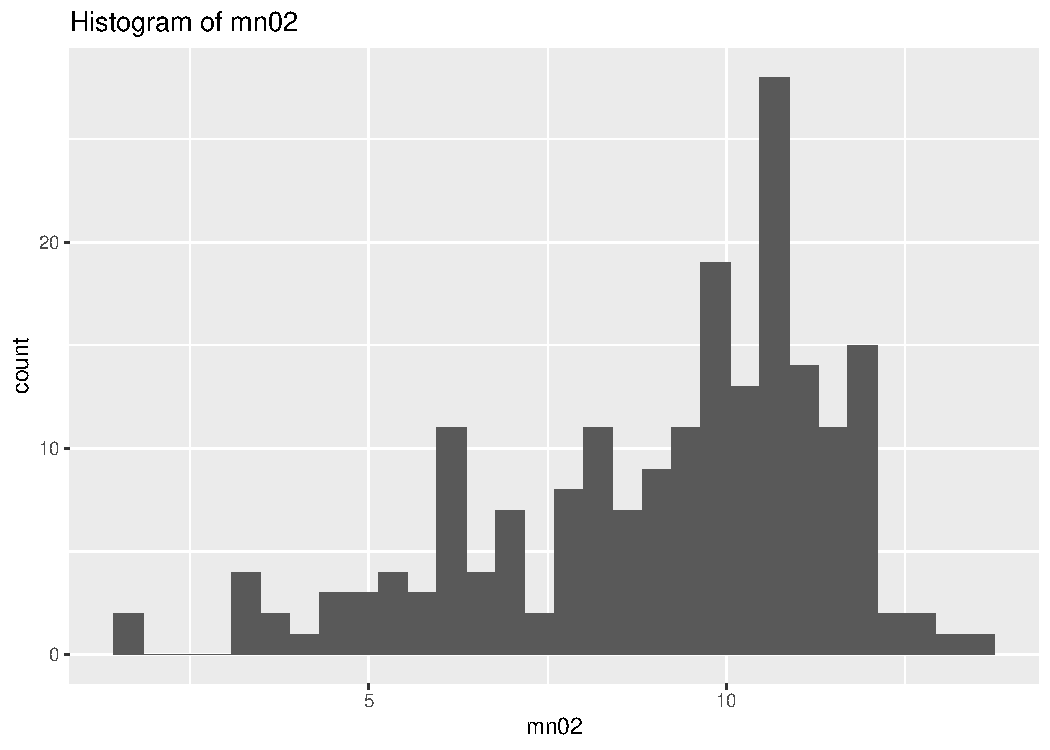
\includegraphics{homework_1_131_files/figure-latex/unnamed-chunk-6-1.pdf}

\begin{enumerate}
\def\labelenumi{\alph{enumi}.}
\setcounter{enumi}{1}
\item
  (1 pts) Add a density curve using geom\_density() and (1 pts) rug
  plots using geom\_rug() to above histogram.
\item
  (1 pts) Create a boxplot with the title `A conditioned Boxplot of
  Algal a3' for a3 grouped by speed. (Refer to help page for
  geom\_boxplot()). (1 pts) What do you notice?
\end{enumerate}

\begin{enumerate}
\def\labelenumi{\arabic{enumi}.}
\setcounter{enumi}{2}
\tightlist
\item
  Dealing with missing values (8 pts in total)
\end{enumerate}

\begin{enumerate}
\def\labelenumi{\alph{enumi}.}
\tightlist
\item
  (2 pts) How many observations contain missing values? (2 pts) How many
  missing values are there in each variable?
\end{enumerate}

\begin{Shaded}
\begin{Highlighting}[]
\CommentTok{\# Counting how many rows contain missing values}
\FunctionTok{sum}\NormalTok{(}\FunctionTok{apply}\NormalTok{(algae, }\AttributeTok{MARGIN =} \DecValTok{1}\NormalTok{, anyNA))}
\end{Highlighting}
\end{Shaded}

\begin{verbatim}
## [1] 16
\end{verbatim}

\begin{Shaded}
\begin{Highlighting}[]
\CommentTok{\#Counting NA values for each variable/column}
\FunctionTok{apply}\NormalTok{(}\AttributeTok{X =} \FunctionTok{is.na}\NormalTok{(algae), }\AttributeTok{MARGIN =} \DecValTok{2}\NormalTok{, }\AttributeTok{FUN =}\NormalTok{ sum)}
\end{Highlighting}
\end{Shaded}

\begin{verbatim}
## season   size  speed   mxPH   mn02     C1    NO3    NH4   cPO4    PO4   CHla 
##      0      0      0      1      2     10      2      2      2      2     12 
##     a1     a2     a3     a4     a5     a6     a7 
##      0      0      0      0      0      0      0
\end{verbatim}

\begin{enumerate}
\def\labelenumi{\alph{enumi}.}
\setcounter{enumi}{1}
\tightlist
\item
  (3 pts) Removing observations with missing values: use filter()
  function in dplyr package to observations with any missing value, and
  save the resulting dataset (without missing values) as algae.del. (1
  pts) Report how many observations are in algae.del.
\end{enumerate}

\begin{Shaded}
\begin{Highlighting}[]
\NormalTok{algae.del }\OtherTok{\textless{}{-}}\NormalTok{ algae }\SpecialCharTok{\%\textgreater{}\%} \FunctionTok{filter}\NormalTok{(}\FunctionTok{complete.cases}\NormalTok{(.))}
\FunctionTok{nrow}\NormalTok{(algae.del)}
\end{Highlighting}
\end{Shaded}

\begin{verbatim}
## [1] 184
\end{verbatim}

\begin{enumerate}
\def\labelenumi{\arabic{enumi}.}
\setcounter{enumi}{3}
\tightlist
\item
  In lecture we present the bias-variance tradeoff that takes the form
  \[\mathbb{E}(y_0-\hat{f}(x_0))^2 = \text{Var}(\hat{f}(x_0))+[\text{Bias}(\hat{f}(x_0))]^2+\text{Var}(\epsilon)\]
  where the underlying model \(Y = f(X) + \epsilon\) satisifes: (1)
  \(\epsilon\) is a zero-mean random noise, and X is non-random (all
  randomness in Y comes from \(\epsilon\)); (2) \((x_0, y_0)\) is a test
  observation, independent of the training set, and drawn from the same
  model; (3) \(\hat{f}(\cdot)}\) is the estimate of f obtained on a
  training set.
\end{enumerate}

\begin{enumerate}
\def\labelenumi{\alph{enumi}.}
\tightlist
\item
  (2 pts) Which of the term(s) in the bias-variance tradeoff above
  represent the reducible error? (2 pts) Which term(s) represent the
  irreducible error?
\end{enumerate}

\(\text{Var}(\hat{f}(x_0))+[\text{Bias}(\hat{f}(x_0))]^2\) is the
reducible error. \(Var(\epsilon)\) represents the irreducible error.

\begin{enumerate}
\def\labelenumi{\alph{enumi}.}
\setcounter{enumi}{1}
\tightlist
\item
  (4 pts) Use the bias-variance tradeoff above to show that the expected
  test error is always at least as large as the irreducible error.
\end{enumerate}

\(\text{Var}(\hat{f}(x_0))\) is always non-negative, and so is the
square of \(\text{Bias}(\hat{f}(x_0))\). As a result, the expected test
MSE is always at least as large as the irreducible error,
\(\text{Var}(\epsilon)\). (Maybe needs more explanation about why Var is
non-negative).

\end{document}
